\section{Related Work}

To take a close look at fault-proneness in object oriented systems, basic oo knowledge is important, as explained in section \ref{content}. The paper "Beyond Language Independent Object-Oriented Metrics: Model Independent Metrics" deals not only with the concept of object orientation but also beyong languages \cite{lanza2002beyond}. The aspects of object orientation such as class, method and attribute can be found here as shown in the following tables, which are subdivided into individual metrics. The meta model from figure \ref{fig0} serves here as a template to understand the relationships between the individual metrics. In the following tables \ref{tab:classmetrics},\ref{tab:methodmetrics} and \ref{tab:attributesmetrics} an excerpt of the metrics is listed. The used meta model and the metrics of the tables allow a multiple extension into different research directions. Thus, they fit the principle of object orientation and serve as a basic template to get into the basic structure of metrics. The advantages of this approach are the increased flexibility, i.e.,
new metamodels can be introduced from any context (for example, the financial world or databases), which provides a standard metric without the need to implement new metrics every time a new context is introduced \cite{lanza2002beyond}. Now, if you look at this system completely from an object orientation perspective, you can see that the basic programming concepts are translated into metrics. Each new method or variable crates more space to generate faults. The complexity of a class is depends, i.e., on the number of methods (NOM) or the number of attributes (NOA), that can be calculated with $(NOA = NIV + NCV)$, as shown in table \ref{tab:classmetrics}. An important metric about the methods of a class is the number of input parameters (NOP) or the number of access on attributes (NMAA), as you can see in figure \ref{tab:methodmetrics}. For the attribute metrics, the number of direct hits is of great importance, as can be found in figure \ref{tab:attributesmetrics}. 

\begin{table}
	\caption{An excerpt of the class metrics from the meta model.}~\label{tab:classmetrics}
	
	\setlength\tabcolsep{3pt}
	\renewcommand{\arraystretch}{1.4}% for the vertical padding
	\begin{tabularx}{\columnwidth}{ | c | p{7cm} | }
		\hline
		Abbrevation & Description \\ \hline\hline
		NHL & Number of classes in superclass chain of class \\ \hline
		NAM & Number of abstract methods \\ \hline
		NCV & Number of class variables \\ \hline
		NIA & Number of inherited attributes \\ \hline
		NIV & Number of instance variables \\ \hline
		NME & Number of methods extended, i.e., redefined in subclass by invoking the same method on a superclass \\ \hline	
		NMI & Number of methods inherited, i.e., defined in superclass and inherited unmodified by subclass\\ \hline
		NOA & Number of attributes $(NOA = NIV + NCV)$ \\ \hline
		NOC & Number of immediate subclasses of a class \\ \hline
		NOM & Number of methods\\ \hline
		PriA & Number of private attributes \\ \hline
		PriM & Number of private methods \\ \hline
		WLOC & Sum of all lines of codes over all methods \\ \hline
		WNI & Number of invocations of all methods \\ \hline
	\end{tabularx}
\end{table}

\begin{table}
	\caption{An excerpt of the method metrics from the meta model.}~\label{tab:methodmetrics}
	
	\setlength\tabcolsep{3pt}
	\renewcommand{\arraystretch}{1.4}% for the vertical padding
	\begin{tabularx}{\columnwidth}{ | c | p{7cm} | }
		\hline
		Abbrevation & Description \\ \hline\hline
		LOC & Method lines of code \\ \hline
		NMA & Number of methods added, i.e., defined in subclass and not in superclass \\ \hline
		MSG & Number of method messages send \\ \hline
		NOP & Number of input parameters \\ \hline
		NI & Number of invocations of other methods within method body \\ \hline
		NMAA & Number of access on attributes \\ \hline
		NOS & Number of statements in method body \\ \hline
	\end{tabularx}
\end{table}

\begin{table}
	\caption{Attribute metrics from the meta model.}~\label{tab:attributesmetrics}
	
	\setlength\tabcolsep{3pt}
	\renewcommand{\arraystretch}{1.4}% for the vertical padding
	\begin{tabularx}{\columnwidth}{ | c | p{7cm} | }
		\hline
		Abbrevation & Description \\ \hline\hline
		AHNL & Class HNL in which attribute is defined \\ \hline
		NAA & Number of times directly accessed \\ \hline
	\end{tabularx}
\end{table}

The limitations of this approach are that not all object-oriented software metrics can be defined in terms of the language independent meta model. Certain metrics tend to be very specialized and are therefore difficult to define in a generic way. Another limitation of this basic concept is that for some metrics, there is it is not yet known how best to define them in a generic way, so the meta model does not include coupling metrics and cohesion metrics.

Fault-Proneness of Open Source Software: Exploring its Relations to
Internal Software Quality and Maintenance Process \cite{kozlov2013fault}. The strengths of our study include the following: 1) we stud-
ied a greater number of metrics than most of the related studies, 2) we studied a greater number of OSS-systems than most
of the studies, and 3) we focused on the fault-proneness of modern Java-based systems and investigated them as an aggre-
gated sample.
ibutes contributing to fault-proneness of open source
software (OSS) can be explained in terms of internal quality
attributes and maintenance process metrics (maintenance
being a phase of the OSS life cycle).
This has been an empirical multiple case study. We have
explored to what extent and how fault-proneness could be
explained by means of internal quality attributes and mainte-
nance process metrics. We first conducted a literature survey
as a basis for taking into account the main findings of other
researchers. Next we analyzed eight OSS systems and their
342 releases.
Software quality was measured in terms of 76 internal
quality attributes, using the static analysis tool SoftCalc.
There were 23 maintenance process metrics obtained from
Source Forge Issue Tracking System (SFITS). Fault-
proneness was measured in terms of Rate of Bug Reports
(RBR) and Average Bug Priority Level (ABPL). That data
was also obtained from SFITS.

The Impact of Accounting for Special Methods in the Measurement of
Object-Oriented Class Cohesion on Refactoring and Fault Prediction
Activities ::: \cite{b4al2012impact}
Class cohesion is a key attribute that is used to assess the design quality of a class, and it
refers to the extent to which the attributes and methods of the class are related. Typically,
classes contain special types of methods, such as constructors, destructors, and access
methods. Each of these special methods has its own characteristics, which can artificially
affect the class cohesion measurement.
This paper empirically explores the impact of including or
excluding special methods on cohesion measurements that were performed using 20
existing class cohesion metrics.
study: The empirical study applies the metrics that were
considered to five open-source systems under four different scenarios, including (1)
considering all special methods, (2) ignoring only constructors, (3) ignoring only access
methods, and (4) ignoring all special methods.
results: he results of
the empirical studies show that the cohesion values for most of the metrics considered
differ significantly across the four scenarios and that this difference significantly affects
the refactoring decisions, but does not significantly affect the abilities of the metrics to predict faulty classes.
This paper empirically addressed whether to include or exclude special methods from
cohesion measurements. Two types of special methods were considered, constructors and
access methods.


Software fault prediction metrics: A systematic literature review ::: \cite{b7radjenovic2013software}. Context: Software metrics may be used in fault prediction models to improve software quality by predict-
ing fault location.
Objective: This paper aims to identify software metrics and to assess their applicability in software fault
prediction. We investigated the influence of context on metrics’ selection and performance.
Method: This systematic literature review includes 106 papers published between 1991 and 2011. The
selected papers are classified according to metrics and context properties.
Results: Object-oriented metrics (49%) were used nearly twice as often compared to traditional source
code metrics (27%) or process metrics (24%). Chidamber and Kemerer’s (CK) object-oriented metrics were
most frequently used. According to the selected studies there are significant differences between the
metrics used in fault prediction performance. Object-oriented and process metrics have been reported
to be more successful in finding faults compared to traditional size and complexity metrics. Process met-
rics seem to be better at predicting post-release faults compared to any static code metrics.
Conclusion: More studies should be performed on large industrial software systems to find metrics more
relevant for the industry and to answer the question as to which metrics should be used in a given
context.In this paper we performed a validation of object-oriented design metrics on a commercial Java system.
The objective of the validation was to determine which of these metrics were associated with fault-
proneness, and hence can be used for predicting the classes that will be fault-prone and for estimating
the overall quality of future systems. Our results indicate that an inheritance and an export coupling
metric were strongly associated with fault-proneness. Furthermore, the prediction model that we
constructed with these two metrics has good accuracy, and the method we employed for predicting the
quality of a future system using design metrics also has a good accuracy.
While this is a single study, it does suggest that perhaps there are a small number of metrics that are
strongly associated with fault-proneness, and that good prediction accuracy and quality estimation
accuracy can be attained. This conclusion is encouraging from a practical standpoint, and hence urges
further studies to corroborate (or otherwise) our findings and conclusions.

\begin{figure}[htbp]
	\centerline{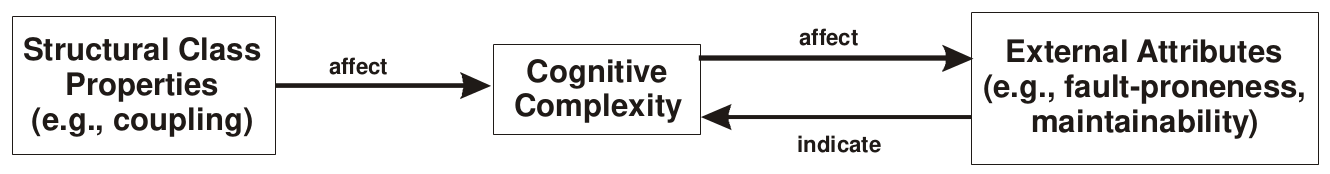
\includegraphics[width=0.5\textwidth]{pictures/faultyclasses1.png}}
	\caption{Theoretical basis for the development of object oriented product metrics \cite{b7radjenovic2013software}.}
	\label{fig3}
\end{figure}

\begin{figure}[htbp]
	\centerline{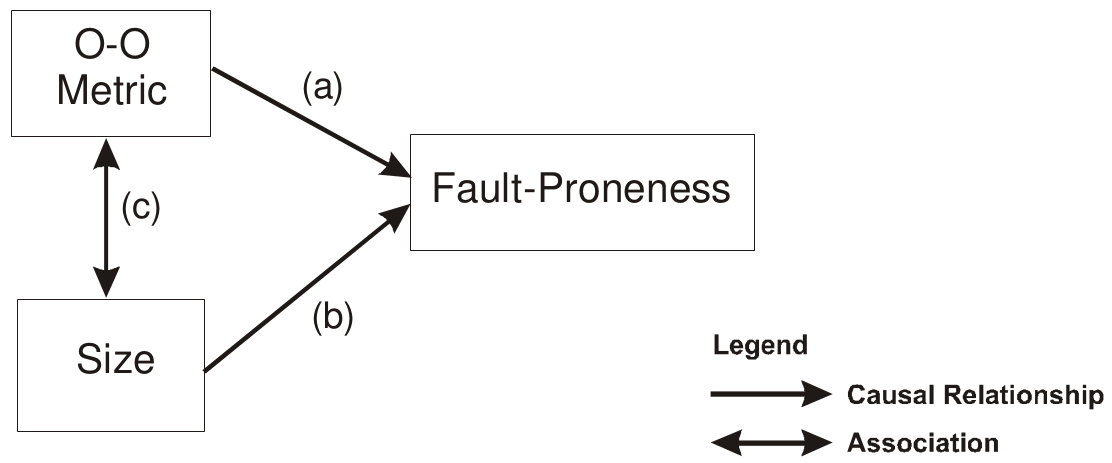
\includegraphics[width=0.45\textwidth]{pictures/faultyclasses2.png}}
	\caption{Path diagram illustrating the confounding effect of class size on the relationship between an object-oriented metric and fault-proneness \cite{b7radjenovic2013software}.}
	\label{fig3}
\end{figure}


A Validation of Object-Oriented Design Metrics as Quality Indicators ::: his paper presents the results of a study in which we empirically investigated the suite of object-oriented design metrics introduced in. More specifically, our goal is to assess these metrics as predictors of fault-prone classes and, therefore, determine whether they can be used as early quality indicators. This study is complementary to the work described in [30] where the same suite of metrics had been used to assess frequencies of maintenance changes to classes \cite{b11basili1996validation}.

The prediction of faulty classes using object-oriented design metrics ::: \cite{b10el2001prediction} Contemporary evidence suggests that most field faults in software applications are found in a small percentage of the software's components. This means that if these faulty software components can be detected early in the development project's life cycle, mitigating actions can be taken, such as a redesign. For object-oriented applications, prediction models using design metrics can be used to identify faulty classes early on. In this paper we report on a study that used object-oriented design metrics to construct such prediction models. The study used data collected from one version of a commercial Java application for constructing a prediction model. The model was then validated on a subsequent release of the same application. Our results indicate that the prediction model has a high accuracy. Furthermore, we found that an export coupling (EC) metric had the strongest association with fault-proneness, indicating a structural feature that may be symptomatic of a class with a high probability of latent faults.


Assessing the Applicability of Fault-Proneness Models Across Object-Oriented Software Projects ::: Furthermore a number of papers have investigated the relationships between metrics of design and the metrics that detect faults in object oriented software. One of the main objectives of this paper is to assess whether fault-proneness models, based on design measurement, are applicable and can be viable decision making tools when applied from one object-oriented system to the other, in a given environment. \cite{b12riand2002assessing}.



- kritische auseinandersetzung, für welche fälle sind welche metriken gut und wieso
- Wann setz ich welche Metriken ein wann im SW Prozess!! und was kann da eintreten passieren
- Auswirkungen von fehlern

Many approaches try to support the software development process with their metrics. All of them work in their own way and in certain situations. 
In order to provide guidance on how to proceed in the software process, some metrics will be explained.